%!TeX spellcheck = en-US
%!TEX root = ../hw1_report.tex
We investigate a primitive version of the Arnoldi method. Let $K_m$ be a matrix representing the Krylov subspace: 
\begin{equation}
K_m = [b, Ab/ \|Ab\|,\dots,A^{m-1}b/ \|A^{m-1}b\|]
\in\mathbb{R}^{n\times m}.
\end{equation}
\subsection{(a)}
The equation
\begin{equation}\label{galerkin}
\mu K_m^TK_mw = K_m^TAK_mw
\end{equation}
\emph{is stemming from the Galerking method applied to the bilinear form associated with the eigenvalue problem $a(u,v) = u^TAv-\mu u^Tv$, with $f(v) = 0$. Prov that \eqref{galerkin} is identical to the approximation generated by Arnoldi's method for eigenvalue problems.}
The Arnoldi method computes an orthogonal basis of $K_m$ such that after $m$ iterations
\begin{equation}
AQ_m = Q_{m+1}H_{\underline{m}}, 
\end{equation}
where $Q_m$ is an orthogonal matrix of size $m$ and $H_{\underline{m}}$ is the corresponding Hessenberg matrix. The eigenvalues of A can then be approximated by the eigenvalues of 
\begin{equation}\label{arnoldi}
Q_m^TAQ_m.
\end{equation}
We use the QR-factorisation of the matrix $K_m$, such that $K_m = Q_mR$. We first show that $R^TR = K_m^TK_m$. Using orthogonality, we have
\begin{equation}\label{eq1}
I = Q^T_mQ_m.
\end{equation}
Multiplying both sides of \eqref{eq1} with $R^T$ and $R$ respectively yields
\begin{equation}
\begin{aligned}
R^T = R^TQ^TQ_m = K^T_mQ_m\Leftrightarrow\\
R^TR  = K^T_mQ_mR = K_m^TK_m.
\end{aligned}
\end{equation}
Now, considering \eqref{galerkin}, we have
\begin{equation}
\begin{aligned}
\mu K_m^TK_mw = K_m^TAK_mw\Leftrightarrow\\
\mu R^TRw = K_m^TAK_mw.
\end{aligned}
\end{equation}
Replacing $K_m$ and $K_m^T$ with the QR-factorisation of $K_m$ yields
\begin{equation}
\mu R^TRw = R^TQ_m^TAQ_mRw.
\end{equation}
Using that $R$ is non-singular, we obtain
\begin{equation}
\mu w = Q_m^TAQ_mw.
\end{equation}
Thus, the approximation computed from \eqref{galerkin} is identical to the eigenvalue approximation obtained from \eqref{arnoldi}, which is what we wanted to show.
\subsection{(b)}
We compare the eigenvalues computed using the Arnoldi method to eigenvalues computed using \eqref{galerkin} after $m$ iterations. Double Gram-Schmidt is used for orthogonalization and the matrix from task 3 is used with $nn=12$ along with a random starting vector $b$. The result is visualised in Figure \ref{res}.
\begin{figure}[h]
\centering
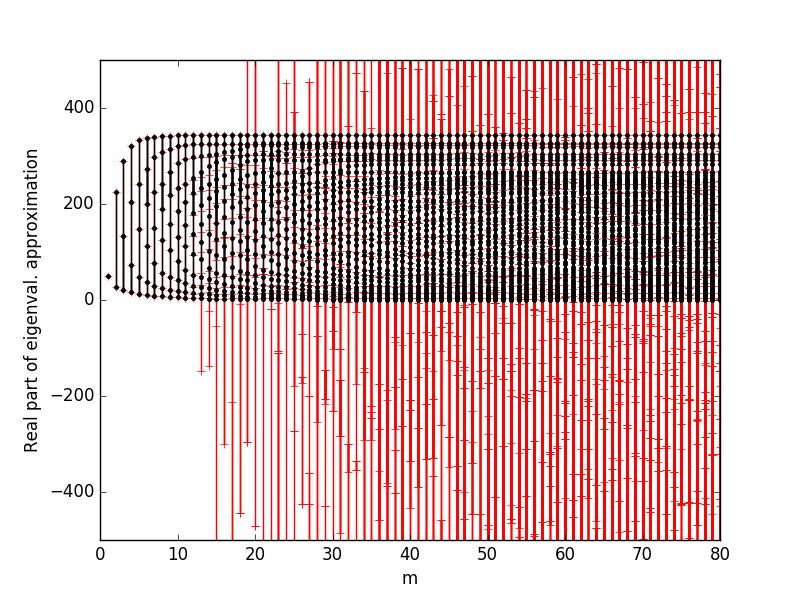
\includegraphics[scale=0.5]{eigenArnoldi.png}
\caption{Comparison of eigenvalues after $m$ iterations.}
\label{res}
\end{figure}
\subsection{(c)}
In exact arithmetic we expect the results from the two approaches to agree. However, forming the Krylov matrices $K_m$ for larger $m$ gives close to singular matrices. As a result of bad conditioning, the Arnoldi approach is to prefer for computing the eigenvalues of the matrix. 
